\begin{frame}{Synchronization}
  What is a Memory Fence?

  \bigskip
  \begin{center}
  \begin{tikzpicture}[scale=0.8,
  thread/.style={blue,very thick,->},
  fence/.style={ultra thick},
  memlocation/.style={thick,draw,fill=blue!20,minimum width=1.5cm},
  write/.style={thick,->,red,dashed},
  read/.style={thick,->,green,dashed},
  meminstr/.style={pos=0.5,font=\small},
  ]
  \only<1-5>{
    \node [memlocation] (mem) at (0,1) { 17 } ;
  }
  \only<6-7>{
    \node [memlocation] (mem) at (0,1) { 18 } ;
  }
  \uncover<+-+(1)>{
    \draw [thread] (-3,5) -- +(0,-1) coordinate (t1write) ;
    \draw [thread] (3,5) -- +(0,-1) ;
  }
  \uncover<+-+(4)>{
    \draw [write] (t1write) -- (mem) node [meminstr] {write 18};
  }
  \uncover<+>{
    \draw [thread] (-3,5) -- +(0,-2) ;
    \draw [thread] (3,5) -- +(0,-2) coordinate (t2read);
  }
  \uncover<.-.(1)>{
    \draw [read] (t2read) -- (mem) node [meminstr] {read};
  }
  \uncover<+>{
    \draw [thread] (-3,5) -- +(0,-3) ;
    \draw [thread] (3,5) -- +(0,-3) coordinate (t2readc);
    \draw [read] (mem) -- (t2readc) node [meminstr] {17};
  }
  \uncover<+>{
    \draw [thread] (-3,5) -- +(0,-4) ;
    \draw [thread] (3,5) -- +(0,-4) ;
  }
  \uncover<+>{
    \draw [thread] (-3,5) -- +(0,-5) ;
    \draw [thread] (3,5) -- +(0,-5) ;
  }
  \uncover<+>{
    \draw [thread] (-3,5) -- +(0,-6) ;
    \draw [thread] (3,5) -- +(0,-6) ;
  }

  \end{tikzpicture}
  \end{center}
\end{frame}
% -----------------------------------------------------------------------------
\begin{frame}{Synchronization}
  What is a Memory Fence? An ordering restriction for memory access.

  \bigskip
  \begin{center}
  \begin{tikzpicture}[scale=0.8,
  thread/.style={blue,very thick,->},
  fence/.style={ultra thick},
  memlocation/.style={thick,draw,fill=blue!20,minimum width=1.5cm},
  write/.style={thick,->,red,dashed},
  read/.style={thick,->,green,dashed},
  meminstr/.style={pos=0.5,font=\small},
  stopped/.style={fill=red,shape=regular polygon,regular polygon sides=8},
  ]
  \draw [fence] (-4,0) -- (4,0) ;
  \only<1-4>{
    \node [memlocation] (mem) at (0,0) { 17 } ;
  }
  \only<5->{
    \node [memlocation] (mem) at (0,0) { 18 } ;
  }
  \uncover<+-+(1)>{
    \draw [thread] (-3,2) -- +(0,-1) coordinate (t1write) ;
    \draw [thread] (3,2) -- +(0,-1) ;
  }
  \uncover<+-+(2)>{
    \draw [write] (t1write) -- (mem) node [meminstr] {write 18};
  }
  \uncover<+-+(3)>{
    \draw [thread] (-3,2) -- +(0,-2) ;
    \draw [thread] (3,2) -- +(0,-2) coordinate (t2read);
  }
  \uncover<+-+(1)>{
    \node [stopped] at (-3,0) {};
    \node [stopped] at (3,0) {};
  }
  \addtocounter{beamerpauses}{2}

  \uncover<+>{
    \draw [thread] (-3,2) -- +(0,-3) ;
    \draw [thread] (3,2) -- +(0,-3) coordinate (t2read);
  }
  \uncover<.->{
    \draw [read] (t2read) -- (mem) node [meminstr] {read};
  }
  \uncover<+->{
    \draw [thread] (-3,2) -- +(0,-4) ;
    \draw [thread] (3,2) -- +(0,-4) coordinate (t2readc);
    \draw [read] (mem) -- (t2readc) node [meminstr] {18};
  }

  \end{tikzpicture}
  \end{center}
  %\uncover<+->{
    %Flavors: All \{reads, writes, accesses\} complete\\
    %before continuing.
  %}
\end{frame}

